\let\negmedspace\undefined
\let\negthickspace\undefined
\documentclass[journal]{IEEEtran}
\usepackage[a5paper, margin=10mm, onecolumn]{geometry}
%\usepackage{lmodern} % Ensure lmodern is loaded for pdflatex
\usepackage{tfrupee} % Include tfrupee package

\setlength{\headheight}{1cm} % Set the height of the header box
\setlength{\headsep}{0mm}     % Set the distance between the header box and the top of the text

\usepackage{gvv-book}
\usepackage{gvv}
\usepackage{cite}
\usepackage{amsmath,amssymb,amsfonts,amsthm}
\usepackage{algorithmic}
\usepackage{graphicx}
\usepackage{textcomp}
\usepackage{xcolor}
\usepackage{txfonts}
\usepackage{listings}
\usepackage{enumitem}
\usepackage{mathtools}
\usepackage{gensymb}
\usepackage{comment}
\usepackage[breaklinks=true]{hyperref}
\usepackage{tkz-euclide} 
\usepackage{listings}
% \usepackage{gvv}                                        
\def\inputGnumericTable{}                                 
\usepackage[latin1]{inputenc}                                
\usepackage{color}                                            
\usepackage{array}                                            
\usepackage{longtable}                                       
\usepackage{calc}                                             
\usepackage{multirow}                                         
\usepackage{hhline}                                           
\usepackage{ifthen}                                           
\usepackage{lscape}
\begin{document}

\bibliographystyle{IEEEtran}
\vspace{3cm}

\title{1-1.3-1}
\author{AI24BTECH11018 - Sreya}
% \maketitle
% \newpage
% \bigskip
{\let\newpage\relax\maketitle}

\renewcommand{\thefigure}{\theenumi}
\renewcommand{\thetable}{\theenumi}
\setlength{\intextsep}{10pt} % Space between text and floats


\numberwithin{equation}{enumi}
\numberwithin{figure}{enumi}
\renewcommand{\thetable}{\theenumi}
\textbf{Problem:}
In triangle \(ABC\), if $\overrightarrow{BA} = 2\mathbf{a}$ and $\overrightarrow{BC} = 3\mathbf{b}$, find $\overrightarrow{AC}$.

\textbf{Solution:}
\begin{table}[h!]
        \centering


\begin{tabularx}{\textwidth}{|X|X|}
\hline
\textbf{Vector} & \textbf{Expression} \\
\hline
$\overrightarrow{BA}$ & 
\[
\begin{bmatrix} 
2.00 \\ 
1.00 
\end{bmatrix} 
\] \\
\hline
$\overrightarrow{BC}$ & 
\[
\begin{bmatrix} 
3.00 \\ 
2.00 
\end{bmatrix} 
\] \\
\hline
$\overrightarrow{AC}$ & 
\[
\begin{bmatrix} 
1.00 \\ 
1.00 
\end{bmatrix} 
\] \\                                         
\hline
\end{tabularx}


        \caption{Input parameters}
\end{table}

\begin{align*}
        \implies \overrightarrow{AC} &= \overrightarrow{AB} + \overrightarrow{BC}, \\
        \implies \overrightarrow{BA} &= 2\mathbf{a}, \\
        \implies \overrightarrow{AB} &= -\overrightarrow{BA} = -2\mathbf{a}, \\
        \implies \overrightarrow{BC} &= 3\mathbf{b}, \\
        \implies \overrightarrow{AC} &= -2\mathbf{a} + 3\mathbf{b}.
\end{align*}
Therefore, the vector $\overrightarrow{AC}$ is: 
\[
\overrightarrow{AC} = 3\mathbf{b} - 2\mathbf{a}.
\]
\begin{figure}[h!]
   \centering
   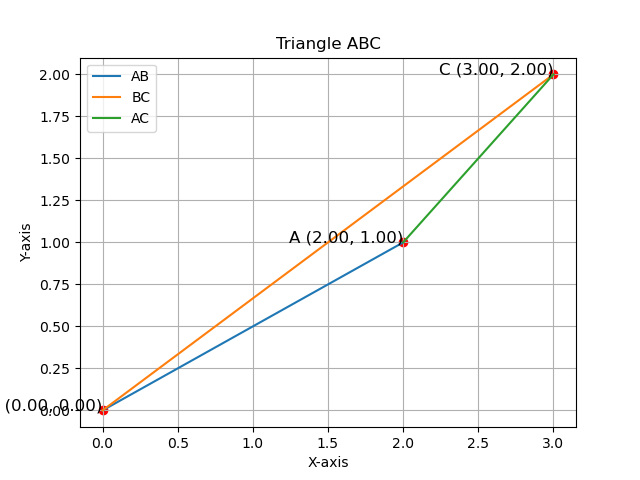
\includegraphics[width=0.7\linewidth]{Triangle_1.png}
   \caption{Triangle}
\end{figure}
\end{document}
